
Given curve  
\begin{align}
    y &= \frac{1}{x-3} , x \neq 3 \label{quadform/78/giveneq}
    \\
    \implies xy - 3y - 1 &= 0
\end{align}

$\therefore$
\begin{align}
    \vec{V} &= \frac{1}{2}\myvec{0 & 1 \\ 1 & 0}
    \\
    \vec{u} &= \frac{-3}{2}\myvec{0 \\ 1}
    \\
    f &= -1
\end{align}

$\because$
\begin{align}
    \abs{\vec{V}} &= \frac{-1}{4}
    \\
    \implies \abs{\vec{V}} &< 0
\end{align}
$\therefore$ \eqref{quadform/78/giveneq} represents a hyperbola .
Now,the characteristic equation of $\vec{V}$ is 
\begin{align}
    \abs{\vec{V} - \lambda\vec{I}} = \mydet{-\lambda & \frac{1}{2} \\ \frac{1}{2} & -\lambda} &= 0
    \\
    \implies \lambda^2 - \frac{1}{4} &= 0
\end{align}
$\therefore$ Eigen values are 
\begin{align}
    \lambda_1 = \frac{1}{2} , \lambda_2 = \frac{-1}{2}
\end{align}
Eigen vector $\vec{p}$ is 
\begin{align}
    \vec{V}\vec{p} &= \lambda\vec{p}
    \\
    \implies (\vec{V} - \lambda\vec{I})\vec{p} &= 0
\end{align}
Eigen vector $\vec{p}_1$ corressponding to $\lambda_1$ can be obtained as
\begin{align}
    (\vec{V} - \lambda_1\vec{I}) &= \myvec{\frac{-1}{2} & \frac{1}{2} \\ \frac{1}{2} & \frac{-1}{2}}\xleftrightarrow[R_1 \leftarrow -2R_1]{R_2 = R_1 + R_2}\myvec{1 & -1 \\ 0 & 0}
    \\
    \implies \vec{p_1} &= \frac{1}{\sqrt{2}}\myvec{1 \\ 1}
\end{align}
Similarly,
\begin{align}
    \vec{p_2} &= \frac{1}{\sqrt{2}}\myvec{-1 \\ 1}
\end{align}
$\therefore$
\begin{align}
    \vec{P} &= \myvec{\vec{p_1} & \vec{p_2}} = \frac{1}{\sqrt{2}}\myvec{1 & -1 \\ 1 & 1}
    \\
    \vec{D} &= \myvec{\lambda_1 & 0 \\ 0 & \lambda_2} = \myvec{\frac{1}{2} & 0 \\ 0 & \frac{-1}{2}}
\end{align}
Now,
\begin{align}
    \vec{c} &= -\vec{V}^{-1}\vec{u} 
    \\
    &= -\myvec{0 & 2 \\2 & 0}\myvec{0 \\ \frac{-3}{2}}
    \\
    &= \myvec{3 \\ 0}
\end{align}
and
\begin{align}
    \sqrt{\frac{ \vec{u}^T\vec{V}^{-1}\vec{u} - f}{\lambda_1}} &= \sqrt{2}
    \\
    \sqrt{ \frac{f- \vec{u}^T\vec{V}^{-1}\vec{u}}{\lambda_2}} &= \sqrt{2}
\end{align}
$\therefore$ Equation of standard hyperbola can be expressed as 
\begin{align}
    \frac{x^2}{2} - \frac{y^2}{2} &= 1
\end{align}
Now,direction vector of tangent with slope = 2 is
\begin{align}
    \vec{m} &= \myvec{1 \\ m} = \myvec{1 \\ 2}
\end{align}
and,normal vector of same tangent is 
\begin{align}
    \vec{m}^T\vec{n} &= 0
    \\
    \implies \vec{n} &= \myvec{2 \\ -1} 
\end{align}
Now,
\begin{align}
    \kappa &= \pm \sqrt{\frac{\vec{u}^T\vec{V}^{-1}\vec{u}-f}{\vec{n}^T\vec{V}^{-1}\vec{n}}}
    \\
    &= \pm \sqrt{\frac{1}{-8}}
\end{align}
$\therefore$ Real value of $\kappa$ does not exist and hence points of contacts of tangent $\vec{q_1},\vec{q_2}$ also does not exist.
\\
Hence,there exists no tangent to the curve having slope = 2.  The hyperbola is plotted in Fig. \ref{quadform/78/fig:hyperbola}.	
%
\begin{figure}[!ht]
\centering
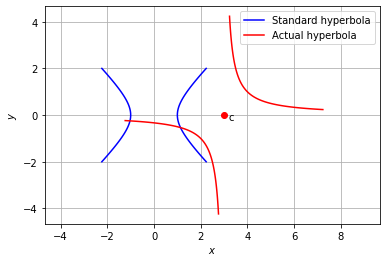
\includegraphics[width=\columnwidth]{solutions/su2021/2/78/Figure8.png}
\caption{Standard and actual hyperbola}
\label{quadform/78/fig:hyperbola}	
\end{figure}


